\documentclass[11pt]{article}

\usepackage[letterpaper,left=1.6in,right=1.6in,top=1.2in,bottom=1.2in]{geometry}

\usepackage[T1]{fontenc}
\usepackage[utf8]{inputenc}

\usepackage{lmodern}
\usepackage{amssymb,amsmath}
\usepackage{graphicx}
\usepackage[11pt]{moresize}

\setcounter{secnumdepth}{0}

%\usepackage[vlined]{algorithm2e}
\usepackage{algorithm,algorithmic}
\usepackage{paralist}
\usepackage{tikz}
\usepackage{xcolor,colortbl}

\begin{document}
\begin{center}
\begin{HUGE}{\bf A6 - Shipping Game}\\ \end{HUGE}
\vspace{10mm}
\begin{LARGE} Contents\\ \end{LARGE}
\noindent\rule{8cm}{0.4pt}
\begin{enumerate} \begin{large}
\item Heap
\item Game Overview
\item Installation
\item Class Explanation
\item Your Tasks
\item Concurrency
\end{large}\end{enumerate}
\end{center}
\newpage

\section{1. Heaps}
As a prologue to Shipping Game, you have to implement a Heap. Heaps are extremely useful data structures that play a vital role in many graph algorithms, including Dijkstra's Algorithm.

Write a class that implements the MinHeap interface and sticks to the given time bounds. To test your code, run the HeapTester main method with your heap implementation classname as an argument. If all of the tests pass, then you're ready to go!

Due to the nature of the project, writing the Heap is a very small part of the project from a conceptual sense. Try to have the heap finished \textbf{one week} after starting the project, so that you have enough time to work on the rest of the project.

TODO: Expand on this section.



\newpage
\section{2. Game Overview}
In Shipping Game (less descriptive name pending) you play the part of a shipping company engineer who makes sure that deliveries get where they're going in a timely fashion. In an instance of Shipping Game, you are presented with an undirected, weighted graph that represents the world. The nodes in this graph are cities where parcels are picked up from or dropped off to, and the edges are highways that connect the cities. Parcels are distributed around the map, each with a starting location (a city in the map) and a delivery destination (a different city in the map).\\
\centerline{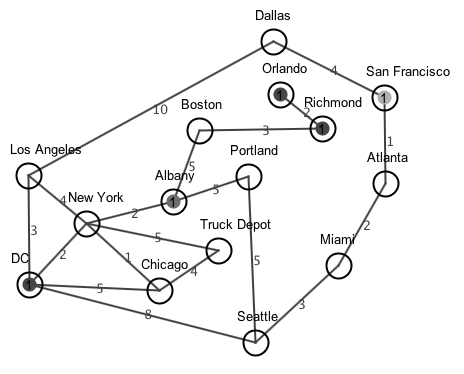
\includegraphics[scale=0.8]{map1.png}}\\
Cities in the map are labeled with their name, highways with their length. The smaller filled-in circles that appear in some cities are parcels that need to be picked up and delivered elsewhere on the map.\\

In order to accomplish this task, you have a fleet of trucks that you are able to control. At the beginning of the game you have the option to give your trucks instructions. Additionally, whenever a truck reaches an important point, such as reaching its destination after traveling a highway, it will let you know so you can give it additional instruction. All Trucks begin the game on the Truck Depot city (there will be exactly one truck depot in every map) and must return there after delivering all parcels for the game to end.

\newpage
\section{3. Installation and Running}
\subsection{Installation}
The code for this project is provided as a .jar file, without source-attachment. Various data files are provided as text files in folders.
\begin{enumerate}
\item Create a new Java project in Eclipse, name it A6.
\item Download ShippingGame.jar and all of the data folders, drag them into your A6 folder. Don't change the names of any of the folders or the code won't be able to find the data.
\item Right click A6 --> Build Path --> Add External Archives --> Select ShippingGame.jar and click Open.
\item Right click A6 -> Build Path --> Configure Build Path... --> Expand ShippingGame.jar by clicking on the triangle to the left of it --> Select Javadoc Location --> Click Edit... --> Select "Javadoc URL" --> Click Browse... --> Select the "doc" folder (don't expand it) and click Open, Click Ok, Click Ok.
\item Create a package in the src folder (right click src --> new... -> package) called \textbf{student}. All code you write for this project must be in the student package.
\item Create a Class in the student package (called whatever you like) that extends \textbf{game.Manager}. Notably, you can't call it Manager. This is your manager class, and is your main submission.
\end{enumerate}

\subsection{Running}
\begin{enumerate}
\item Select A6 -> Run As... --> Run Configurations... --> New Launch Configuration (blank page with star in top left)
\item Click Search... next to Main class --> Select game.main
\item Switch to the Arguments tab --> Enter the name of your manager class that you created in the student class in the top text box. No .java necessary, just the name of the class.
\item Click run.
\item From here on out, the settings are saved, so you can simply run the project by clicking the green run button as usual.
\end{enumerate}

\subsection{Arguments}
You can provide additional arguments to the runner to have it do different things. All argument combinations have to start with the name of your manager. With just the manager classname provided, the game will launch in GUI mode. There are no other applicable arguments for this mode. Any other combination of arguments will launch the game in GameRunner mode instead, where the game will automatically run your manager on a sequence of maps. 

To run GameRunner on a series of seeds <seed1> <seed2> <seed3> such as $15, 12345, 907230587$, use each seed as an argument, separated by a space. (replace MyManager with the name of your Manager):
\begin{center}
MyManager 15 12345 907230587
\end{center}
To run GameRunner on a series of $n$ random seeds, use the $-r$ flag, followed by the number of random seeds to run (replace MyManager with the name of your Manager). For example, to run your manager on 10 random seeds:
\begin{center}
MyManager -r 10
\end{center}
The GameRunner mode includes the GUI to show the progression of the run games. It also prints output of the games to the console. If you would like to just see the output and not show the GUI (headless), add the $-h$ tag. Thus, either:
\begin{center}
MyManager -h 15 12345 907230587
\end{center}
or
\begin{center}
MyManager -h -r 10
\end{center}
\begin{figure}[h]
\centerline{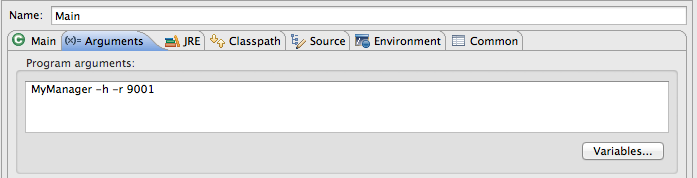
\includegraphics[scale=0.65]{args.png}} 
\caption{\em{Running MyManager in headless mode on 9001 random seeds.}}
\end{figure}


\newpage
\section{4. Class Explanation}
Assuming your installation worked correctly, you should be able to see the javadoc specifications for all of the public methods available to classes in the game package. If not, consult section 2 of this guide or ask on Piazza/at office hours.\\
The game structure follows the below diagram.
\begin{figure}[h]
\centerline{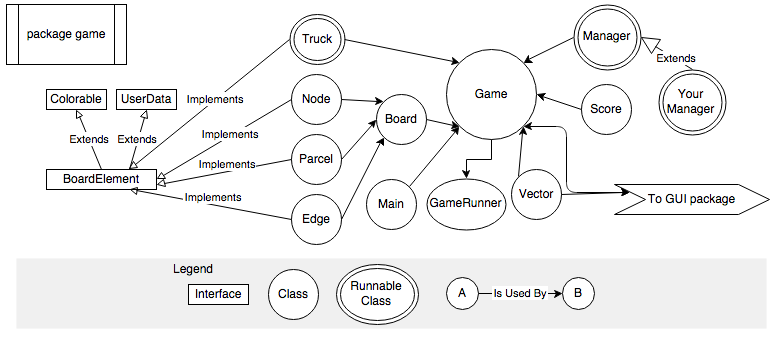
\includegraphics[scale=0.7]{hirearchy.png}} 
\end{figure}
\\Each interface and class in the figure is briefly explained below. For a more thorough  explanation or the method list of a certain interface or class, see the javadoc spec for that interface or class.
\subsection{Colorable}
The colorable interface is implemented in classes that have a "color". Pertaining to ShippingGame, BoardElement extends Colorable so that all elements that are drawn on the map are guaranteed to have a color.
\subsection{UserData}
The UserData interface is implemented in classes that allow the user (Your Manager) to store data in them. You don't have to use this feature of classes that implement UserData, but it may prove useful in some graph algorithms.
\subsection{BoardElement}
In addition to being a concatenation of the requirements of the Colorable and UserData interfaces, the BoardElement interface specifies required behaviors for displaying an object on the GUI. Implementing classes are required to be able to provide various GUI-sensitive information, such as how to draw it, what it's name on the GUI is, and if there are any trucks currently "on it".
\subsection{Truck}
Instances of the Truck class are the game pieces of ShippingGame. Trucks take instructions from Managers, are able to travel the map and pick and drop off a single parcel at a time. Trucks are runnable - each instance of truck is set to run in its own thread.
\subsection{Node}
Instances of the Node class make up the Board. Each Node in the map represents a city that is connected to other cities by highways (Edges). Nodes store parcels until a truck picks them up. One special Node is designated as the TruckDepot, where all Trucks begin the game and must return to before the game can end.
\subsection{Edge}
Instances of the Edge class connect the Nodes in the Board. Each Edge represents a highway that connects two cities (Nodes). Edges in ShippingGame are undirected (bidirectional) and weighted (have length). The weight of the edge tells how long it takes for a truck to travel a given Edge - higher weight takes longer to travel.
\subsection{Parcel}
Instances of the Parcel class are the scoring pieces of ShippingGame. Parcels start at a certain Node on the Board, and award points when they are successfully delivered to their destination Node. The game can only end once all of the Parcels have been delivered.
\subsection{Board}
The Instance of the Board for each game stores the Nodes, Edges, and Parcels associated with the game. It has the scoring constants related to various actions taken during the game, and convenience methods such as getting a random Node or random Edge.
\subsection{Score}
The Instance of Score for each game encapsulates the score for the game. In addition to preventing the user (Your Manager) from altering the score, it has convenience methods for checking for a valid color and calculating the cost of a given Truck Speed.
\subsection{Vector}
The Vector class is very similar to the Point class built into java, except that it allows for doubles in all of its calculations rather than restricting to integers. It is used internally for calculation and is provided to you for convenience.
\subsection{Main}
The Main class begins execution of the game, and stores static convenience methods for use all over the project.
\subsection{Manager}
The Manager class is abstract - it is up to you to extend it. The non-abstract behavior of the Manager class gives convenience methods for getting the map, trucks, and parcels associated with the game. It also gives the Notification enum, which specifies the different reasons a Truck would notify the Manager of a change.
\subsection{Game}
An instance of the Game class represents the game as a whole. The game class is the unifying factor that ties all of the other pieces together, along with communicating with the GUI to make sure the visual version of the game is up to date. It includes convenience methods for querying the current state of the game.
\subsection{Game Runner}
An instance of the Game Runner class allows the automatic running of many games. This is useful to automatically test your manager on may different board, and can be accessed via arguments given to main.
\subsection{Your Manager}
An instance of Your Manager fills in the missing behavior of the Manager class to determine how the game runs. See the next section for more on what you have to do in your extension of the Manager class.

\newpage
\section{5. Your Tasks}
In order to complete the assignment, your primary task is write a class extending the abstract Manager class explained in the previous section. In order to do this, you will have to override and implement the two abstract methods declared in the Manager class: \textbf{run()} and \textbf{truckNotification(Truck t, Notification message)}. These two methods determine the behavior of the trucks in the game. On their own, trucks don't do anything; it's up to you to instruct them.\\

\begin{figure}[h]
\centerline{
\includegraphics[scale=0.4]{fry.jpg}} 
\caption{\em{The average intelligence of your shipping boys}}
\end{figure}

run() is called by the game as soon as the game begins, and allows you to do initial computation and give your trucks their initial set of instructions. Additionally, the body of run() will run in a separate thread from all of the trucks, so you can continue to do computation after the trucks have begun their travel. Your implementation can either loop forever and continually add information to the trucks or execute a single time for initial instructions and then rely on the truckNotification method for further interaction.\\

truckNotification(Truck t, Notification message) is called by trucks whenever they do something of note. For a full list of the reasons why a truck would call this method, see Manager.Notification in the previous section and in the javadoc. This method is called by the truck in its own thread in order to ask for more instructions. For example, upon arrival at a new node in the graph, the truck may send a notification that there is at least one parcel at the current node. Perhaps you want that truck to pick up that parcel before continuing on its route.

\newpage
\section{6. Concurrency}
TODO

\end{document}